\chapter{Algorithms and Implementation}

The currently implemented and algorithmized parts of the intermediate language are the following: the formal intermediate language (parametric timed regular expression), a parametric timed automaton implementation, a mapping between the two, and a prototype automaton executor.

\section{Parametric Timeout Regular Expression}

Currently the regular expression has a grammar implemented in Xtext, which generates a textual editor, and can parse textual input to an EMF model. This EMF model can be transformed later. 
The grammar is shown on \cref{lst:grammar}. \todo{Wrong cref}

Note that the parameter listing is inside with square brackets ``[]'' to make the language context free. If we would use the simple round brackets, then A(B) would be ambiguous -- it could be either an A event with a B parameter, or a simple sequence of event A and event B with an unnecessary bracket.
\todo{Do we require additional explanation?}

\section{Parametric Timed Event Automaton}

The parametric timed automaton was implemented using Eclipse Modeling Framework to provide a metamodel for it. The entire static structure is represented with EMF objects, but some of the runtime concepts are not covered with this metamodel, this will be further explained in \cref{section:algo:paramhandling}.

\subsection{Finite Automaton}

The subset of the metamodel which represents the Finite Automaton functions are shown on \cref{fig:algo:basic_automaton}.
The event automaton logic is represented by the State, Transition, and EventGuard classes.
Every State has a boolean flag to show whether it is an acceptor state or not, and have any number of incoming and outgoing transitions.
Transitions have one EventGuard which shows what type of event can fire the transition. 

\begin{figure}[h]
	\centering
	\includegraphics[width=\linewidth]{figures/chapter_5/Basic_automaton_diagram}
	\caption{Metamodel of the Event Automaton}
	\label{fig:algo:basic_automaton}
\end{figure}

\subsection{Timeout Event Automaton}

The additional classes required to implement the Timeout functionalities are shown on \cref{fig:algo:timed_automaton}.
Every timed expression in the regular expression is compiled to SymbolicTimer. Upon entering such timed region all transitions will have a SetTimerAction Action to start the timer. The transitions which exit the given region will have a ResetTimerAction Action for that timer. Every state which is in the Timeout region will have a Transition with a SymbolicTimeoutEvent instead of a SymbolicInputEvent to further specify the movement of the token in case of timeout. Currently these SymbolicTimeoutEvent Transitions are always pointing on a Trap state, however as this gives a more generalized automaton structure so this can help in the future to make the implementation of the Timeout Event Automaton with Intervals easier.

A scratch of the implementation plan is duplicate the entire region, for each timeout \\ $\langle \mathit{Complex Pattern} \rangle_{t_0 < t < t_1}$ compile the $\mathit{ComplexPattern}$ twice. For the sake of easier understanding, let us call the first compilation's result  pre-interval as it represents when the token is before the desired time interval, and the call the second compilation result in-interval as it represents when the token is in the desired time interval. For each state in the pre-interval part the transition with the timeout will point to the equivalent state in the in-interval part, and for each state in the in-interval part the transition with the timeout will point to a trap state. All of the transitions, which would point to the accepting state of the pre-interval should be pointed to a Trap State as these shows that the pattern match occurred before the required interval.
  
\begin{figure}[h]
	\centering
	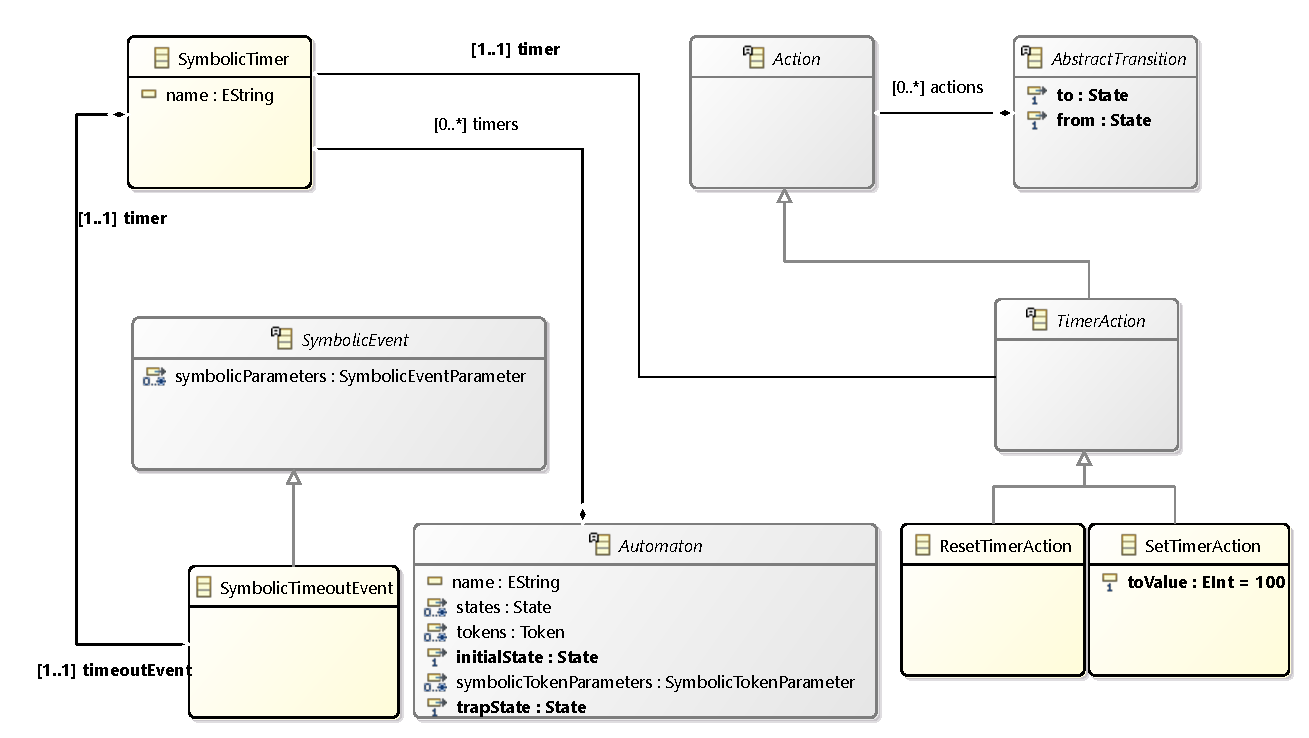
\includegraphics[width=\linewidth]{figures/chapter_5/Timing_diagram}
	\caption{Metamodel of the Timed Event Automaton}
	\label{fig:algo:timed_automaton}
\end{figure}

\subsection{Parameters and Bindings}
\label{section:algo:emfparameterhandilng}

The part of the automaton metamodel which is extended with the parametric properties are shown on \cref{fig:algo:parametric_automaton}
The parametrization of the events is represented by the Parameter abstract class. The type of each parameter is implemented with a reference to a SymbolicEvent instance. Parameters can be Fix or Free, an Event only has Fix parameters, but the tokens can have both. Event parameters can be bound to fix values or to a token parameter, this is done by the ConstantBinding and TokenParameterBinding respectively.

This parameter handling approach is not the best, however this is which can be easily implemented using EMF.
The deeper analysis of these parameter relations can are discussed in \cref{section:algo:paramhandling}.

\begin{figure}[h]
	\centering
	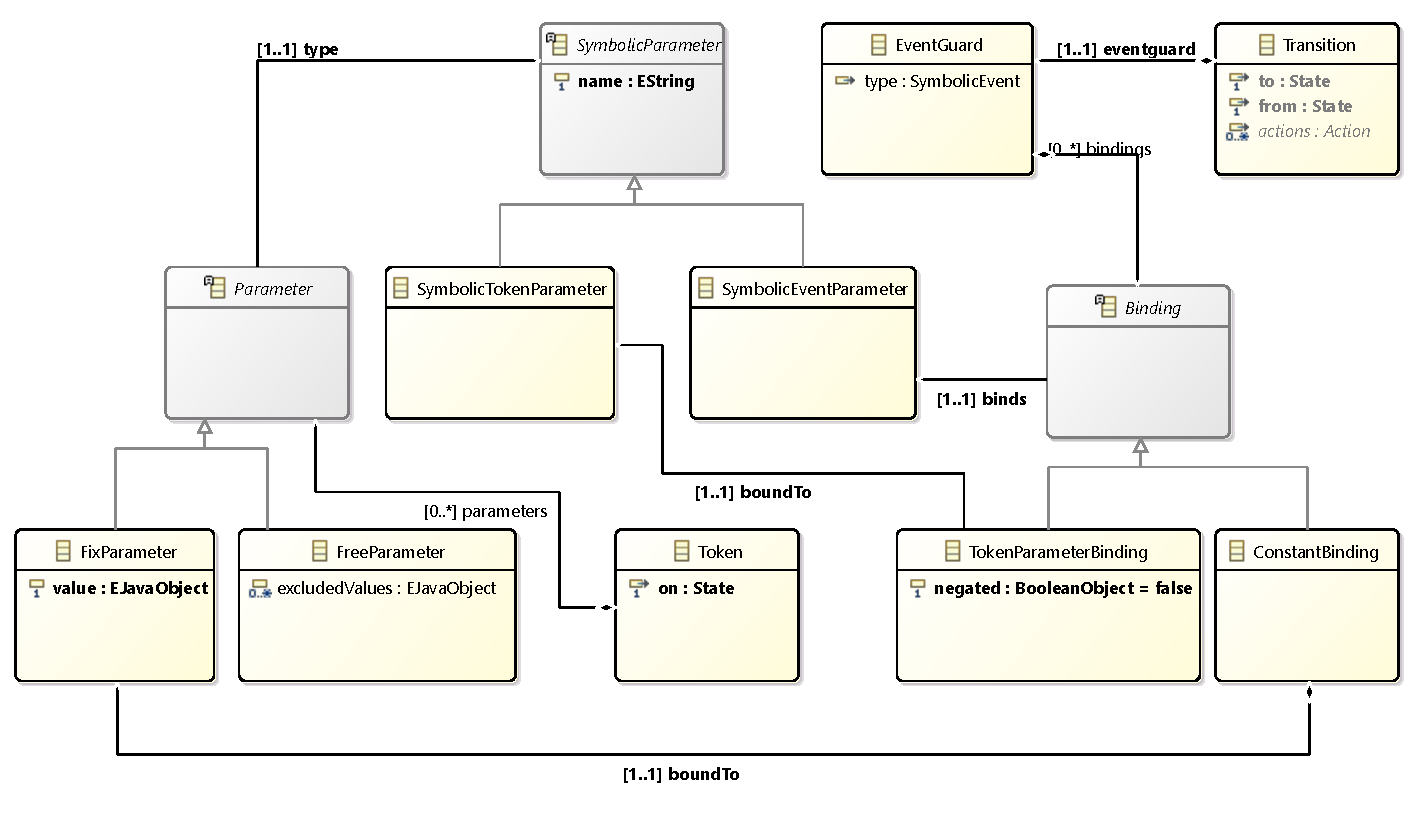
\includegraphics[width=\linewidth]{figures/chapter_5/Parameters_diagram}
	\caption{Metamodel of the Parametric Timed Event Automaton}
	\label{fig:algo:parametric_automaton}
\end{figure}

\section{Transformation from VEPL to the intermediate language}

Regular expressions can be built from VEPL patterns, taking the event contexts into consideration
Strict immediate is show on \cref{tab:cep:vepl_regex_strict}, and Chronicle is shown on \cref{tab:cep:vepl_regex_chronicle}.
Each of the patterns must start with a $\Sigma^*$, as in Complex Event Processing every pattern might have arbitrary prefix.

Note that the semantics introduced in the previous chapter for the OR operator of Regular Expression, and the semantics of VEPL defined in\citep{davidi} are not exactly the same.

\begin{table}
	\caption{Basic VEPL operators in strict immediate context, expressed with regular expressions}		
	\label{tab:cep:vepl_regex_strict}
	\centering
	\begin{tabular}{@{}ll@{}}
		\toprule
		VEPL operator             & Regular Expression \\ \midrule
		$p_1$ $\rightarrow$ $p_2$ & $p_1\; p_2$        \\
		$p_1$ OR $p_2$            & $p_1|p_2$          \\
		$p\{\ast\}$               & $p^*$              \\
		$p[t]$                    & $p[t]$             \\ \bottomrule
	\end{tabular}
\end{table}

\begin{table}
	\caption{Basic VEPL operators in chronicle context, expressed with regular expressions}		
	\label{tab:cep:vepl_regex_chronicle}
	\centering
	\begin{tabular}{@{}ll@{}}
		\toprule
		VEPL operator             & Regular Expression               \\ \midrule
		$p_1$ $\rightarrow$ $p_2$ & $p_1 \; (\Sigma/(p_2))^* \; p_2$ \\
		$p_1$ OR $p_2$            & $p_1|p_2$                        \\
		$p\{\ast\}$               & nothing                          \\
		$p[t]$                    & $p[t]$                           \\ \bottomrule
	\end{tabular}
\end{table}

\section{Automaton Executor}
	Two approaches exist on executing a parametric timed automaton, and in both ways there are multiple tokens in each automaton, so in some sense both can be considered nondeterministic.
	However from the token's point of view we can consider the two approaches deterministic and a nondeterministic.
	
%	In  both ways there are multiple tokens in the automaton with one parameter relation each, therefore they can be both considered nondeterministic.
	
	\paragraph{Deterministic Execution}
	In the deterministic approach the automaton should not contain any $\varepsilon$-edges and a ``token can go only one way'', or more formally, there is only one transition for each token to fire. 
	In this case every token moves exactly one on each event, splitting the potential bindings to two part, one which matched the event's parameter, and one which did not.
	
	\paragraph{Nondeterministic Execution}
	\todo{Maybe pseudocode}
	In the nondeterministic way, the automaton can contain $\varepsilon$-edges, and a token can move through multiple transitions each. This solution implies an another way to handle the parameters, as the executor should do the following steps:
	\begin{enumerate}
		\item Save each token in a list,
		\item Find the enabled transitions,
		\item For each of the enabled transitions, create a parameter relation according to the event,
		\item Compute the intersection of each token with each enabled transitions which is an outgoing transition of the state which the token is on,
		\item Move each intersected token parameter binding to the state where the transitions point,
		\item Move these tokens through the $\varepsilon$-closure, applying any actions to the moved parameters,
		\item And remove the old tokens which were saved in the first step.
	\end{enumerate}

	On the implementation level the Nondeterministic Executor has been implemented as it is more general can execute any automaton generated from the regular expressions.

	\todo{Maybe an example execution?}


%	The algorithm first searches for all the activated transitions.
%	If it finds an activated transition, it iterates over the tokens which in on that state. The first token with matching (non-confronting) parameter list will be split to the next state if there are new parameter bindings from the event, or moved if there are no new bindings.
%	If a token enters an acceptor state it will trigger a callback function.
	

	\subsection{Parameter Handling}
	\label{section:algo:paramhandling}
	
%	Parameter handling can be done with two approach, either we consider the execution deterministic or nondeterministic.
%	In both cases each token requires a ``ParameterRelation''.
%	But these parameter relation requires different Interface depending on the style of the execution:

	The required operations on the Parameter Relations are:
	\begin{itemize}
		\item If the execution is deterministic, the following operations are required:
			\begin{itemize}
				\item $P_1 = P_1 \cup P_2$, i.e.~a relation can be added to another with mutating the first one,
				\item $P_1 = P_1 \setminus P_2$, i.e.~a relation can be removed from an another with mutating the first one,
				\item can be checked if it is empty,
				\item and add every possible parameter value with $\forall$.
			\end{itemize}
		\item However if the execution is considered nondeterministic, an other set of operation is required:
			\begin{itemize}
				\item $P_1 \cup P_2$, i.e.~two relation's union can be computed,
				\item $P_1 \cap P_2$, i.e.~two relation's intersection can be computed,
				\item can be checked if it is empty,
				\item and add every possible parameter value with $\forall$.
			\end{itemize}
	\end{itemize}

	The ``add every possible parameter value'' is only required upon the initialization of the automaton, and considering that the relations are empty on construction this operation can be changed to a complementer operation, which is more general.
	In both cases the union is required for further optimization, and not an absolute necessity.

	\subsection{Most Na\"ive approach}
	
	The most na\"ive approach is to keep every potential binding in the memory, for example if there is a pattern $a[i_1]\;b[i_1,\dots,i_n]$ where all parameters are integers and event $a[1]$ happens the state of the memory is shown on \cref{tab:algo:memory}. This indicates that there would be $2^{32^{n-1}}$ objects in the memory, which is not feasible even if $n=3$.\footnote{If each object's size is just 1 bit even then $n=2$ would waste 512MB of memory}
	
	\begin{table}
	\caption{State of the memory on the most na\"ive approach}		
	\label{tab:algo:memory}
	\centering
	\begin{tabular}{ccccc}
		\toprule
		$i_1$ &  $i_2$   &  $i_3$   & \dots &  $i_n$   \\ \midrule
		  1   &    0     &    0     & \dots &    0     \\
		  1   &    1     &    0     & \dots &    0     \\
		  1   &    0     &    1     & \dots &    0     \\
		  1   &    1     &    1     & \dots &    0     \\
		      &          &  \vdots  &       &  \\
		  1   &    1     &    1     & \dots &    1     \\
		  1   &    2     &    0     & \dots &    0     \\
		  1   &    2     &    1     & \dots &    0     \\
		      &          &  \vdots  &       &  \\
		  1   &    2     &    1     & \dots &    1     \\
		  1   &    2     &    2     & \dots &    0     \\
		      &          &  \vdots  &       &  \\
		  1   & $2^{32}$ & $2^{32}$ & \dots & $2^{32}$ \\ \bottomrule
	\end{tabular}
	\end{table}
	
	\subsection{Na\"ive approach}	

	The na\"ive approach is to keep an abstract value for each parameter for each token,
	where the abstract value can be either be
	\begin{itemize}
		\item A concrete value, which shows that for that token the given parameter is bound to that value, i.e.~the given parameter must be exactly that value, or
		\item a list of excluded values which shows that for that token the given parameters values have been reduced by them, i.e.~the given parameter must not be any of the excluded values
	\end{itemize}

	With this approach, every operation seems to be plausible, however a simple counter-example easily shows that the solution can not support the deterministic approach.
	Consider the following example:
	\begin{enumerate}
		\item At first we have a parameter relation $P$, where $\langle p_1 = \forall, p_2 = \forall \rangle$, i.e.~with two excluded values with empty exclusion list.
		\item If the relation $R$, $\langle p_1 = 1, p_2 = 1 \rangle$ is subtracted from $P$, $P$ would be reduced to $\langle p_1 = \forall \setminus \{1\}, p_2 = \forall \setminus \{1\} \rangle$.
		\item If the relation $S$, $\langle p_1 = 2, p_2 = 2 \rangle$ is subtracted from $P$, $P$ would be reduced to $\langle p_1 = \forall \setminus \{1, 2\}, p_2 = \forall \setminus \{1, 2\} \rangle$.
		\item The problem occurs when we would try to subtract the relation $\langle p_1 = 2, p_2 = 1 \rangle$ as it \emph{should} be in the relation, but it is not. 
	\end{enumerate}

	\subsection{Decision List}
	
	A decision list is a list of data, where each cell contains either a concrete value or the symbol $\ast$ which stands
	for ``anything''. To find out if a values in the relation the rows must be read in order, and find the first row which conforms the values you are searching for \todo{algorithm} \dots and return the containment.
	An example of a decision list is shown on \cref{tab:cep:decision_list}
	
	\begin{table}
		\centering
		\caption{An example of a Decision List}		
		\label{tab:cep:decision_list}
		\begin{tabular}{cccc}
			\toprule
			\# & containment &  $A$   &  $B$   \\ \midrule
			1  &     $+$     &  $2$   & $\ast$ \\
			2  &     $+$     &  $3$   &  $5$   \\
			3  &     $-$     & $\ast$ & $\ast$ \\ \bottomrule
		\end{tabular}
	\end{table}

	\subsection{Disjunctive Decision Set}

	An event -- in a more formal way -- is a conjunction of a logical statement. When we think of $\mathit{Allocate}(1,2)$ we actually mean that we have an event called $\mathit{Allocate}$ where $\mathit{Task} = 1 $ $\with$ $\mathit{Resource} = 2$.
	With this mindset we can assume that a Parameter Binding Relation is actually only a disjunction of such statements.
	
	An example of Disjunctive Decision Set is shown on \cref{tab:cep:dds}.
	
	\begin{table}
		\centering
		\caption{An example of a Disjunctive Decision Set}		
		\label{tab:cep:dds}
		\begin{tabular}{ccc}
			\toprule
			containment &  $A$   &          $B$           \\ \midrule
			    $+$     &  $2$   & $\ast\setminus\{1,2\}$ \\
			    $+$     &  $3$   &          $5$           \\
			    $-$     & $\ast$ &         $\ast$         \\ \bottomrule
		\end{tabular}
	\end{table}

	\subsection{MDDe}
	
	MDDe is a Multiple-value Decision Diagram with else branches. We could use simple MDD's with intervals, but in many cases the parameters do not have a supremum and infimum and they are not in a sequence.
	

	
	\subsection{Additional Data Structures}
	
	There are many more data structures which can be used for the underlying implementation of a Parameter Relation. Two more was under consideration, Trie, and BDD. Both are somewhat similar to MDD, however Trie is a mutable data structure, which theoretically seems to be more efficient in the case of the Deterministic Execution, as the operations are always mutating the data structure. The other one was BDD which is the Binary version of MDD, but thanks to that, the tree structure would be higher, however with a lower branching factor, and updating such data structures could be cheaper than using MDDs.
	
	\section{Preliminary measurements}
	To analyze the efficiency of the implementation some measurements were done, using the example from \cref{chap:cep}.
	
	\subsection{Measurement setup}
	As the current implementation lacks of logical clocks, and the timed properties can only be evaluated by elapsing the required time, the pattern $a[i] \; a[i]^\ast \; r[i] \; r[i]^\ast \; a[i]$ will be the parametric and not temporal example.
	The scalability is viewed from three points:
	
	\begin{enumerate}
		\item How well does the implementation scale with the size of the pattern?
		\item How well does the implementation scale with the size of the input sequence?
		\item With a given pattern and a given size for the input sequence, does it matter how many times the automaton accepts?
	\end{enumerate}
	
	To answer the first question, the pattern must be extended. The extension was with adding one more requirement to the pattern: How much is the maximum allocation allowed for one process. Therefore the extended pattern will be $ ( a[i] \; a[i]^\ast \; r[i] \; r[i]^\ast \; a[i] ) | (a[i],\dots,a[i])$, where on the right side of the pattern the length sequence of $a[i]$ events will be expanded to one, ten, one hundred, one thousand, and ten thousand.
	
	To answer the second question, input sequences were generated in five sizes: one long, ten long, one hundred long, one thousand long and ten thousand long ones.
	However to measure multiple cases, these inputs are generated with the following logic:
	\begin{enumerate}
		\item A randomly generated sequence,
		\item only events $a[1]$ and $a[2]$ but on a random sequence to not a match, in other words to generate less than the required $a[1]$ events and $a[2]$ events,
		\item only sequences of $a[1] r[1] a[1]$ and $a[2] r[2] a[2]$ to have as much matches as possible.
	\end{enumerate}

	The measurements were done with two underlying parametric data structures MDDe, and the  Disjunctive Decision Set.
	
	
		\subsubsection{Threats to validity}
		Every measurement was done thirty two times. The first two measurement result was dropped as it was considered as the warm up for the JVM. From the remaining thirty, the median was calculated, to have a stable value which is the least affected by the noises of the measurement and the extremely high or low values. Between every iteration of a measurement, the garbage collector was called three times followed by a sleep to ensure that the garbage collection is if required.
		
		The measurements were aimed to cover some part of most use cases, however they are not exhausting every potential use case to think of.
		
		
	
	\subsection{Measurement Results}
		Compilation time: 
	
		\todo{Diagram}
		
		\todo{Explanation}
	
	
	%Research Questions: Itemize q1-q2, Performance
	%
	%Regex -> Automata
	%or Execution
	%
	%
	%Measurement setup
	%What kind of input, what kind of queries, what was exactly measured, number of runs (min 5, ideally 30), median/min
	%Measure +2 times and throw away the first.
	%
	%1 min runtime limit.
	%
	%
	%/section{Measurement Results}
	%Diagrams: explanation: explicity state the scalability 
	%analysis of the result a1-a2-a3: answer q1-q2-q3
	%
	%
	%Threats to validity : Eclipse is running, on my machine, noises expectedly cancelled with median (but who knows)
	%Only one stuff was measured but this hűen reprezentálja a problémát
	%Nagyon függ a bemeneti querytől és csak szemléltetni tudjuk a skálázhatóságot
	%
	%
	%System.Nanosec
	%
	%Minden java indításkor belemegítés
	%
	%Minden mérés után 3x System.GC (Threats to validity)
	%Thread.sleep(3s)
	
	